\let\negmedspace\undefined
\let\negthickspace\undefined
%\RequirePackage{amsmath}
\documentclass[journal,12pt,twocolumn]{IEEEtran}
\usepackage[utf8]{inputenc}
\usepackage{graphicx}
\usepackage{amsmath}
\usepackage{mathrsfs}
\usepackage{txfonts}
\usepackage{stfloats}
\usepackage{bm}
\usepackage{cite}
\usepackage{cases}
\usepackage{subfig}
\usepackage{amsfonts}
\usepackage{amssymb}
\usepackage{enumitem}
\usepackage{mathtools}
\usepackage{tikz}
\usepackage{circuitikz}
\usepackage{verbatim}
\usepackage[breaklinks=false,hidelinks]{hyperref}
\usepackage{listings}
\usepackage{calc}
\usepackage{float}
\usepackage{longtable}
\usepackage{multirow}
\usepackage{multicol}
\usepackage{color}
\usepackage{array}
\usepackage{hhline}
\usepackage{ifthen}
\usepackage{chngcntr}

\newcommand{\BEQA}{\begin{eqnarray}}
	\newcommand{\EEQA}{\end{eqnarray}}
\newcommand{\define}{\stackrel{\triangle}{=}}
\bibliographystyle{IEEEtran}
%\bibliographystyle{ieeetr}
\def\inputGnumericTable{}
\let\vec\mathbf
\providecommand{\pr}[1]{\ensuremath{\Pr\left(#1\right)}}
\providecommand{\sbrak}[1]{\ensuremath{{}\left[#1\right]}}
\providecommand{\lsbrak}[1]{\ensuremath{{}\left[#1\right.}}
\providecommand{\rsbrak}[1]{\ensuremath{{}\left.#1\right]}}
\providecommand{\brak}[1]{\ensuremath{\left(#1\right)}}
\providecommand{\lbrak}[1]{\ensuremath{\left(#1\right.}}
\providecommand{\rbrak}[1]{\ensuremath{\left.#1\right)}}
\providecommand{\cbrak}[1]{\ensuremath{\left\{#1\right\}}}
\providecommand{\lcbrak}[1]{\ensuremath{\left\{#1\right.}}
\providecommand{\rcbrak}[1]{\ensuremath{\left.#1\right\}}}
\providecommand{\abs}[1]{\left\vert#1\right\vert}
\providecommand{\res}[1]{\Res\displaylimits_{#1}}
\newcommand{\myvec}[1]{\ensuremath{\begin{pmatrix}#1\end{pmatrix}}}
\newcommand{\mydet}[1]{\ensuremath{\begin{vmatrix}#1\end{vmatrix}}}
\newcommand{\solution}{\noindent \textbf{Solution: }}
\title{Assignment 4}
\author{PRABHAV SINGH\\BT21BTECH11004}
\date{}
\begin{document}
	% make the title area
	\maketitle
	\begin{abstract}
		This document contains the solution to Question 4 of exercise 16.3 of Chapter 16 (Probability) in the NCERT Class 11 Textbook.
	\end{abstract}
	
	\textbf{Probability Excercise 16.3 Q4.}\\
	A card is selected from a pack of 52 cards.
	\begin{enumerate}[label=(\roman{enumi})]
		\item How many points are there in the sample space?
		\item Calculate the probability that the card is an ace of spades.
		\item Calculate the probability that the card is an ace.
		\item Calculate the probability that the card is black.
	\end{enumerate} 
	\solution Let $X\in \cbrak{0,1,2}$ is a random variable that denotes outcome of the experiment, where $X = 0$ denotes occurrence of an ace card of spades, $X = 1$ denotes occurrence of an ace card, $X = 2$ denotes occurrence of a black card.
	\begin{enumerate}
		\item Total number of points in sample space\\
		\begin{align}
		  n(S) = 52 
		  \end{align}
			In PMF approach :
		\begin{align}
			\pr{X = r} = {n\choose r}\times p^{r} \times (1-p)^{n-r} 
		\end{align}
		\item Probability that the card is an ace of spades, for this $  n=1 ,r=1 , p=\frac{1}{52} $
		\begin{align}
			\pr{X = 0} &= {1\choose 1}\times (\frac{1}{52})^{1} \times (1-\frac{1}{52})^{1-1} \\
			&= \frac{1}{52}
		\end{align}

		\item Probability that the card is an ace card, for this $  n=1, r=1 ,p=\frac{4}{52}  $
		\begin{align}
			\pr{X = 1} &= {1\choose 1}\times (\frac{4}{52})^{1} \times (1-\frac{4}{52})^{1-1}  \\
			&=\frac{1}{13}
		\end{align}
		\item Probability that the card is black, for this $  n=1, r=1 ,p=\frac{26}{52}  $
		\begin{align}
			\pr{X = 2} &= {1\choose 1}\times (\frac{26}{52})^{1} \times (1-\frac{26}{52})^{1-1}\\
			&=\frac{1}{2}
		\end{align}
	\begin{figure}[!ht]
		\centering
		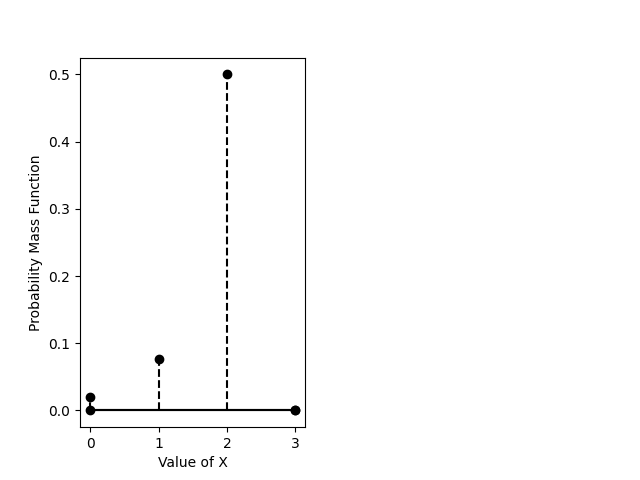
\includegraphics[width=\columnwidth]{C:/Users/prabh/AI1110 ASSIGNMENTS/Assignment 4/Figure/pmf2.png}
		\caption{Plot of the PMF}
		\label{fig:pmf}
	\end{figure}
		
	\end{enumerate}
\end{document}
